\documentclass[a4paper,11pt]{jsarticle}


% 数式
\usepackage{amsmath,amsfonts}
\usepackage{bm}
% 画像
\usepackage[dvipdfmx]{graphicx}


\begin{document}

\title{デコーダ回路の設計と制作}
\author{古城隆人}
\date{\today}
\maketitle

\newpage
\section{目的}
電子天秤の制作を行うにあたり、値を表示させるために7セグメントLED1の表示回路を作成する。デコーダ回路の入力は、セレクタ回路から3bitの信号を受け取る。
\section{原理}
実際に回路の制作を行うにあたって使用する部品と動作原理を説明する。
\subsection{ブレッドボード}
ブレッドボードを使用し、デコード回路の作成を行う。この部品はジャンパ線を使用して自由に回路を組み替えれるので、回路の制作に適している。
ブレッドボード上で配線するときはショートしているピンについて理解をしないといけない。
図\ref{fig:breadboard}にブレッドボード写真を示す。
\begin{figure}[h]
  \centering
  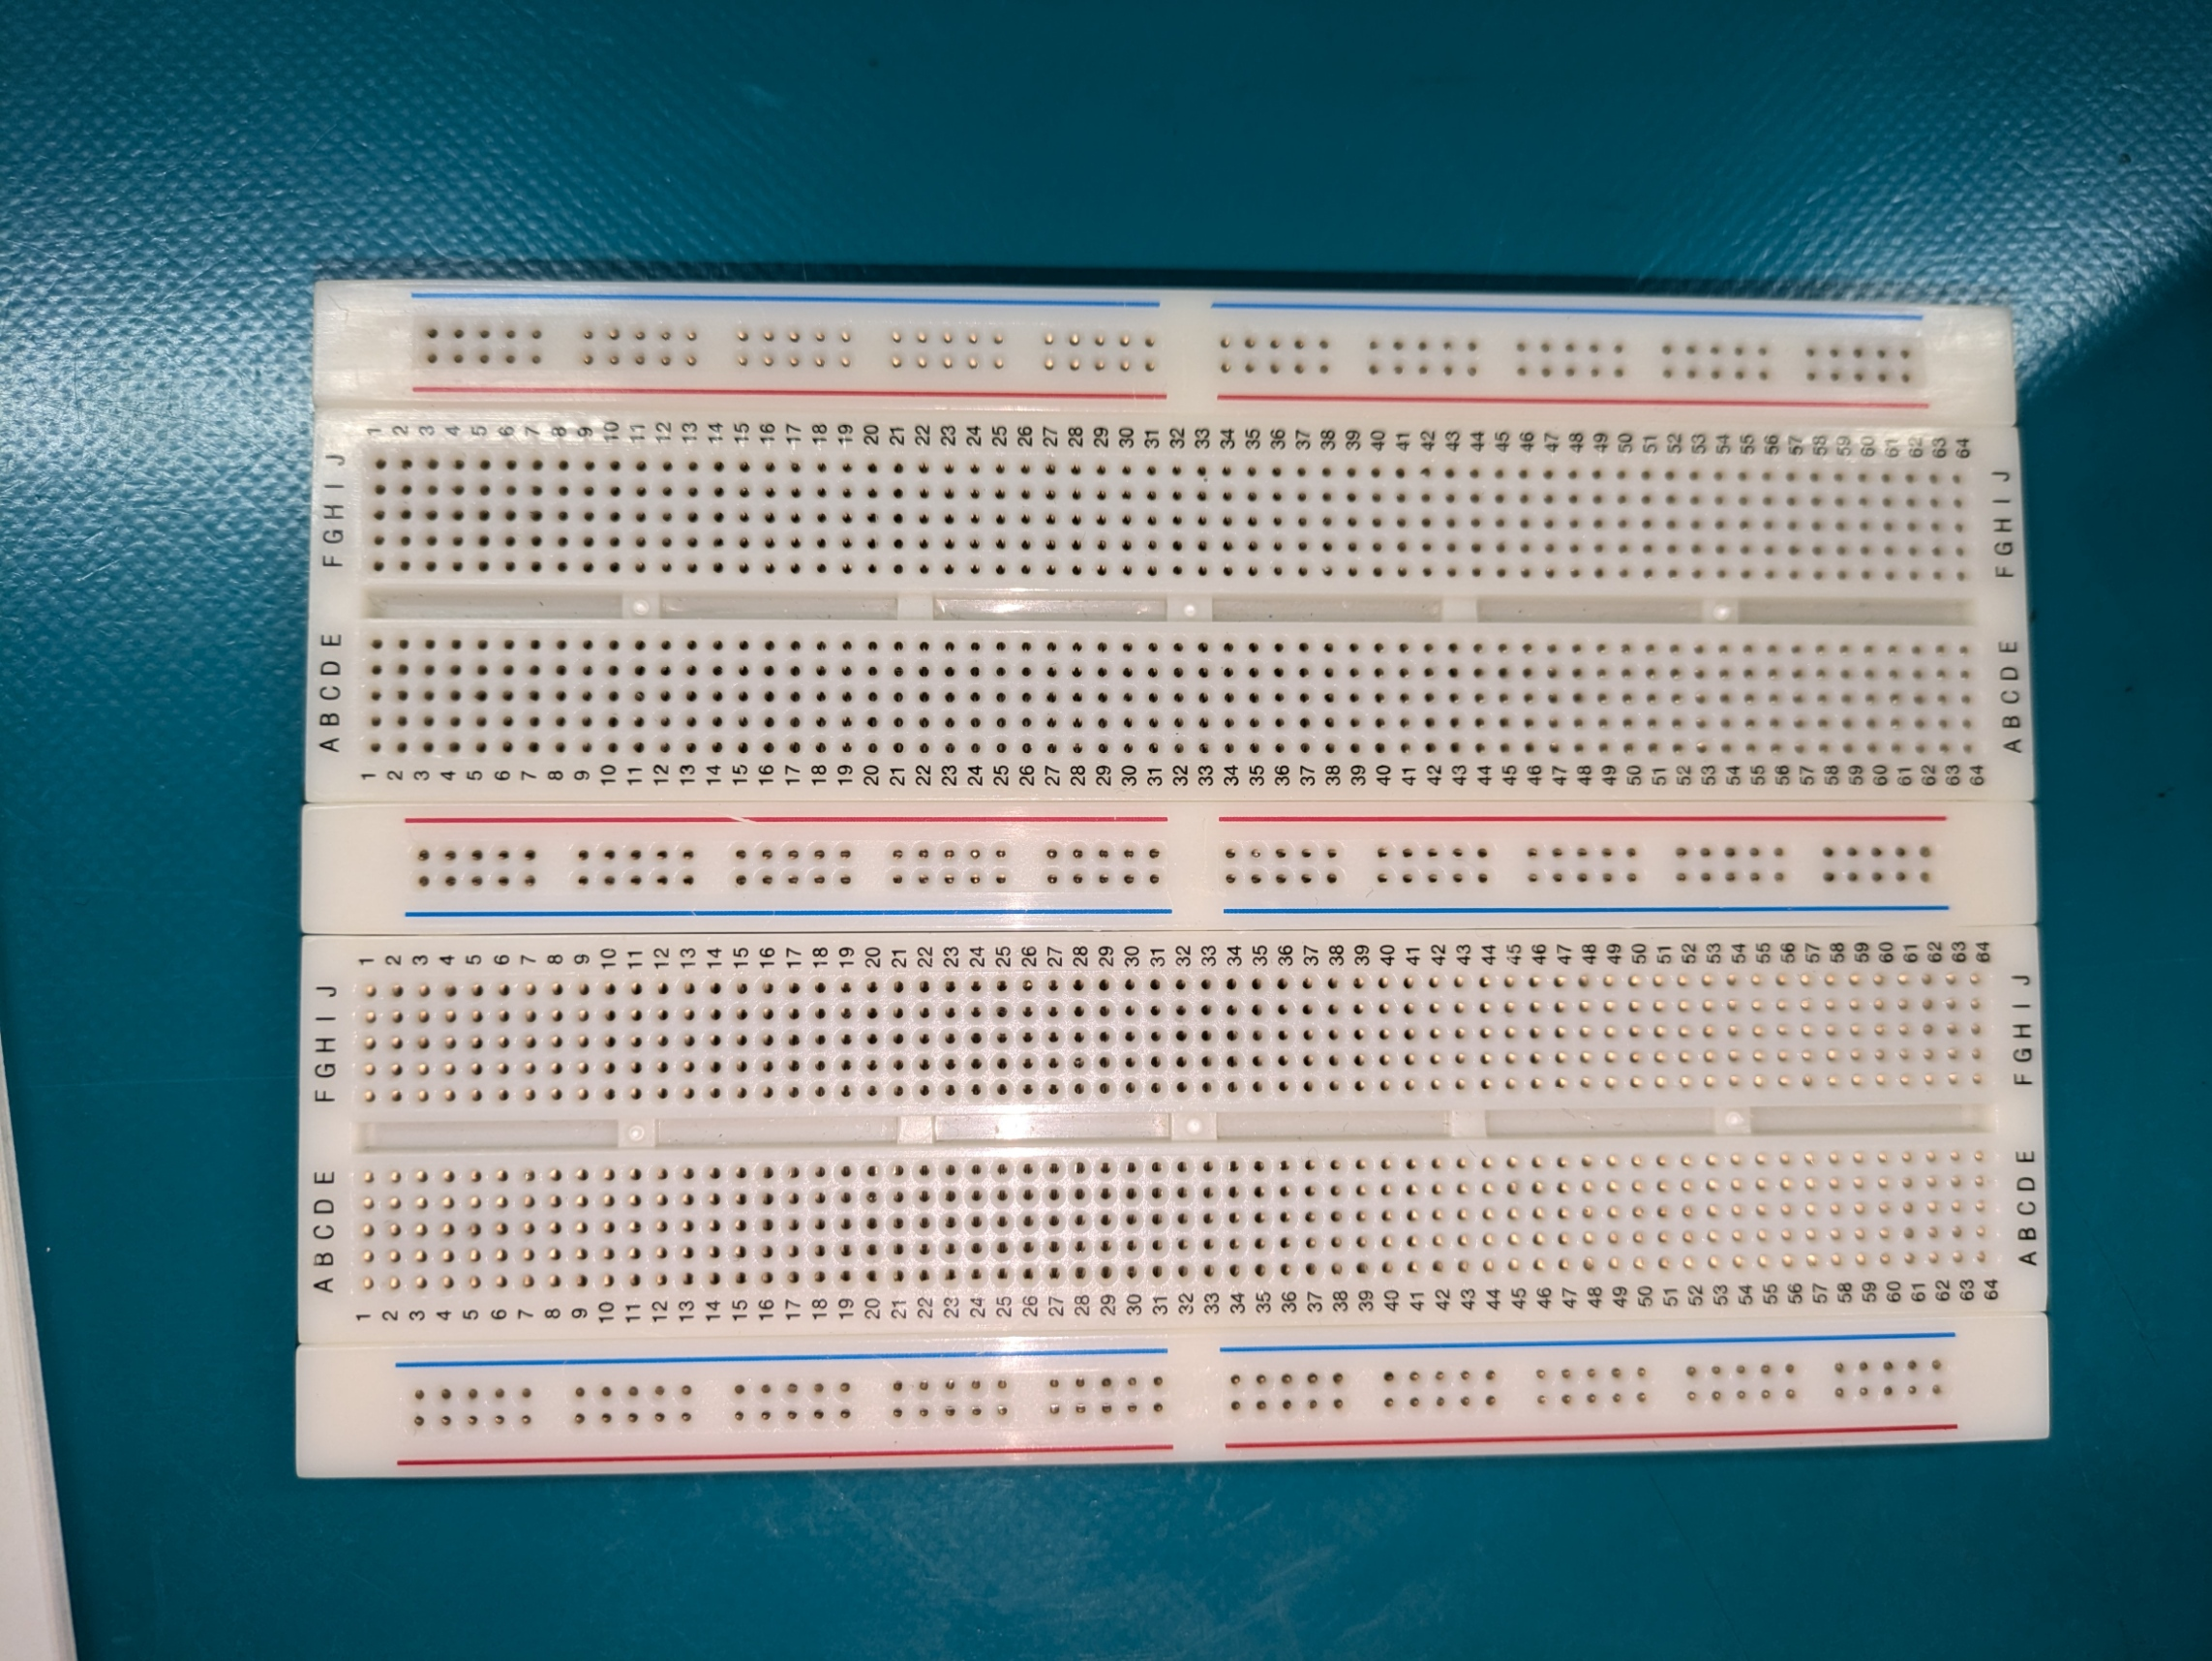
\includegraphics[width=10cm]{./images/breadboard.jpg}
  \caption{ブレッドボードの内部構造}
  \label{fig:breadboard}
\end{figure}
このブレッドボードは5個の部品に分かれており、2この穴が縦に空いてる場所が3個ある。それの間に10個の穴が縦に空いて真ん中に溝がある部品がある。
3個ある横長の部品は内部で電気的に横につながっており、それは青色と赤色の線が横に書いてある穴同士がつながっている。
個の基板では横に2本の線があるので真ん中のピン同士の電気的なつながりはない。この部品は主に電源の端子として使用される。
今回は青色の線が描かれているところを$GND$、赤色の線が描かれているところを$+5V$として使用する。
2個ある長方形の部品は縦にショートしており、5個の穴が内部で電気的につながっている。真ん中の溝で電気的なつながりは切れている。
そのためこのブレッドボードは縦に5個つながっている穴が縦に4個配置されている。この部品は主にIC、ジャンパ線を挿して回路を作成する部品である。
\subsection{7セグメントLED}
7セグメントLEDは7つのLEDを組み合わせたもので、数字を表示させる用途で使用する。7つのLEDはそれぞれaからgまでの名前がついており、それぞれのLEDを点灯させることで数字を表示させる。
7セグメントLEDの略図を図\ref{fig:7seg}に示す。基本的に一番上から時計回りにaからgまでのLEDが配置されている。
\begin{figure}[h]
  \centering
  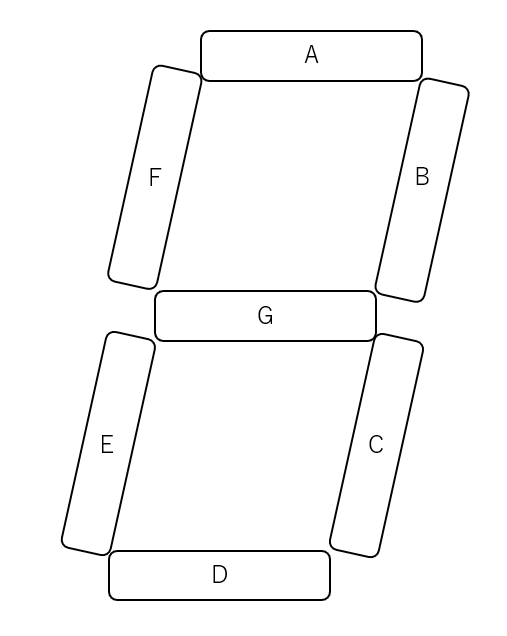
\includegraphics[width=10cm]{./images/7seg.png}
  \caption{7セグメントLEDの略図}
  \label{fig:7seg}
\end{figure}
今回使用するLEDはアノードコモン型の7セグLEDを使用する。アノードコモン型では、その名の通りLEDのアノード端子が共有になっている。
LEDのアノードとは、電流が入力される方向の端子であり、電流を出力する端子をカソードという。アノードからカソードに電流を流すことによりLEDを光らせることが出来る。
そのため、7セグLEDの各LEDの端子とアノードコモンのピンで電圧差が生じたらLEDが光る。アノードコモンのピンには今回は5Vをつなぐため、
各LEDのピンには $GND$ を接続すると光らせることが出来る。
7セグLEDのピン配置を図\ref{fig:7segpin}に示す。
左下のピンから反時計回りに1から10までのピンがあり、3,8がアノードでそれ以外がカソードに接続している。
\begin{figure}[h]
  \centering
  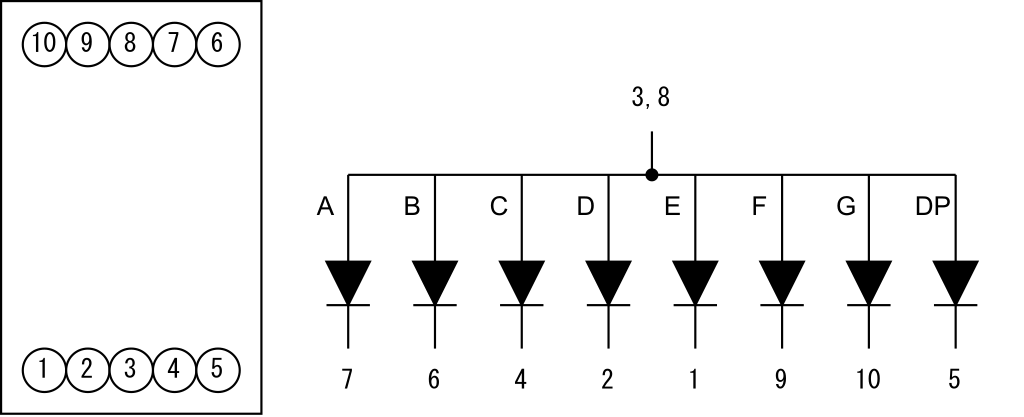
\includegraphics[width=10cm]{./images/7segpin.png}
  \caption{7セグメントLEDのピン配置}
  \label{fig:7segpin}
\end{figure}
\subsection{汎用ロジックIC}
汎用ロジックICでは、論理演算を行うことが出来る回路部品である。2進数の情報を基に7セグLEDの光らせ方を制御するのに使用する。
論理演算ではAND / ORなどがある。例えばAND演算では2本の信号がHIGH($+5V$)の時に出力がHIGHになる。これはどちらも1であるためである。
論理回路の入力と出力を示したものを真理値表という。表の列の数だけ変数があり、入力/出力、場合によっては内部の状態を示す。
AND、OR、NOT、XORの真理値表を表\ref{tab:logic}に示す。今回ではA、Bが入力で、AND、OR、NOT、XOR、が出力である。
この0 1はそれぞれLOW($GND$)、HIGH($+5V$)を示している。
\begin{table}[h]
  \centering
  \caption{論理演算の真理値表}
  \begin{tabular}{|c|c|c|c|c|c|c}
    \hline
    A & B & AND & OR & NOT (A) & NOT (B) & XOR \\
    \hline
    0 & 0 & 0 & 0 & 1 & 1 & 0 \\
    0 & 1 & 0 & 1 & 1 & 0 & 1 \\
    1 & 0 & 0 & 1 & 0 & 1 & 1 \\
    1 & 1 & 1 & 1 & 0 & 0 & 0 \\
    \hline
  \end{tabular}
  \label{tab:logic}
\end{table}
ICでは内部の特徴に違いがあり、それを名前で表している。今回使用するICは74LSシリーズである。
74LSシリーズはバイポーラトランジスタを使用している。
\textbf{ICの出力端子}
ICには論理回路に入出力があるように、入出力するための端子がある。その内部の構造として、出力端子を説明する。
ICの内部は複数のトランジスタで構成されている。
トランジスタとはスイッチのようなもので、ベースとエミッタの電位差によってコレクタとエミッタ間の電流を制御できる。
トランジスタにはNPN型とPNP型の2種類があるが今回はNPN型で説明を行う。
NPN型トランジスタの特性はベースとエミッタ間に電流が流れる、ようは電位がベースのほうが大きくなるとコレクタからエミッタにかけて電流が流れる。
図 \ref{fig:transistor}では、Bをベース、Cをコレクタ、Eをエミッタとしている。
図 \ref{fig:transistor}(a)にICの出力端子の一個前のイラストを示す。右側の四角いでっぱりが出力端子で内部に書かれているものが出力の一個前のトランジスタである。
図 \ref{fig:transistor}(b)にトランジスタの特性を示す。ベースとエミッタ間に電流が流れるとコレクタとエミッタ間に電流が流れる。そのため出力端子に電流が流れないため、出力はLOWとなる。
この出力の先に電流が流れるかもしれないが、この先に接続するICの内部抵抗よりもトランジスタの抵抗のほうが小さいのでエミッタに電流が流れる。
図 \ref{fig:transistor}(c)では、ベースとエミッタが同じ電位にあるため、コレクタからエミッタにかけて電流が流れない。そのため出力端子の先に違う電位があれば電流が流れる。
IC内部で発生するこれらの電流のことを前者をシンク電流、後者をソース電流という。
\begin{figure}[h]
  \centering
  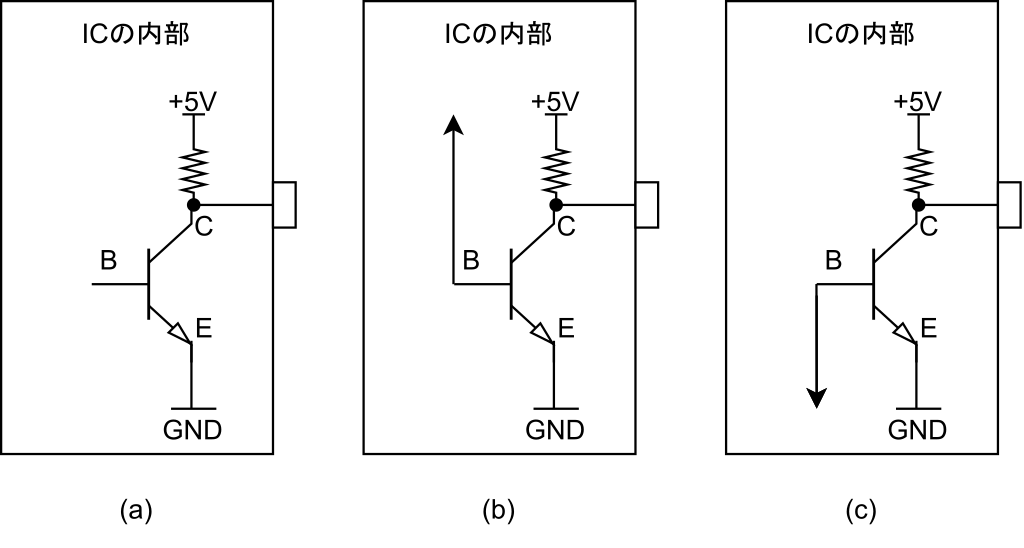
\includegraphics[width=10cm]{./images/trans.png}
  \caption{トランジスタの特性}
  \label{fig:transistor}
\end{figure}
ICによって真紅電流、ソース電流の値が異なるのでデータシートで確認を行い、電子回路を組むことが出来るのかを把握する必要がある。
例えば今回ではアノードコモンのLEDを制御するため出力端子にLEDのカソードを接続し、シンク電流を流すことでLEDを光らせる。
そのため、$I_{ol}$の電流を確認する必要がある。$I_{ol}$はシンク電流、$I_{oh}$はソース電流である。
\textbf{ICの入力端子}
汎用ロジックICではピン番号が同じように命名されている。今回使用するICは74LS04(NOT)、74LS08(AND)、74LS32(OR)、74LS86である。
いずれも14ピンのDIP型のICである。DIPとはDual Inline Packageの略称であり、パッケージの表面にくぼみがあるのが特徴である。
このくぼみがあるほうを表、端子が出てるほうが裏である。表の状態でくぼみを上にした時に、左上から反時計回りに1から14までの数字が命名されている。
74シリーズでは7番に$GND$、14番に$+5V$を接続する。それ以外の端子は入出力端子である。
\section{実験方法}

\section{結果}

\section{考察}

\section{付録}


\end{document}